\section{Use of Motion Primitive in Skill Based Framework}
\label{apx:skill based framework}
Similar to the concept that speech consist of syllables , it has been observed
that tasks in can be broken down into smaller elements which are called as
skills. The skills in turn can be decomposed of smaller atomic movements called
as Motion Primitives. A  three layer Framework was introduced by
\cite{pedersen_robot_2015} and is illustrated in figure \ref{skill framework}.



\begin{figure}[htp]
\centering
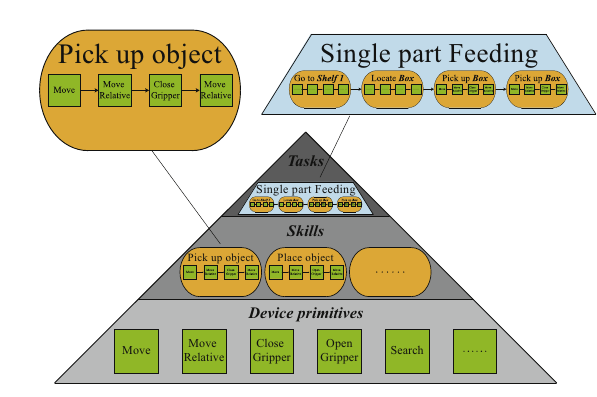
\includegraphics[scale=0.5]{images/skill_framework.png}
\caption[Skill based framework]{Three layers of primitives, skills and tasks. The components in each layer is essentially a combination of lower layer. \cite{pedersen_robot_2015}}
\label{skill framework}
\end{figure}

The three layers of the framework are :
\begin{itemize}
    \item Motion Primitives
    \item Robotics Skills
    \item High Level Tasks
\end{itemize}

\subsection{Motion Primitives}
The lowest layer is the called the motion primitives. It consist of atomic
movement.

\subsection{Robotics Skills}
Robotic skills form the base of the skill based Framework. Robotic skills are
object-centred robot abilities, which can be easily parametrized.
  
% subsection  (end)

\subsection{High level Tasks}
The Higher level description of a task to be done. Ususally in this layer
planners like \acrfull{strips} or \acrfull{pddl} are used to choose which robotic skills has to be
executed.

% section  (end)

The proposed motion primitive approach fits exactly inside the skill based 
framework mentioned here.
The motion primitives can be combined together and higher level skills
can be executed.

